\documentclass[tikz]{standalone}
\usetikzlibrary{arrows, positioning}
\usetikzlibrary {arrows.meta}
\usepackage{xcolor}
\definecolor{allcolor}{RGB}{148,182,233}
\newcommand*{\equal}{=}
\begin{document}
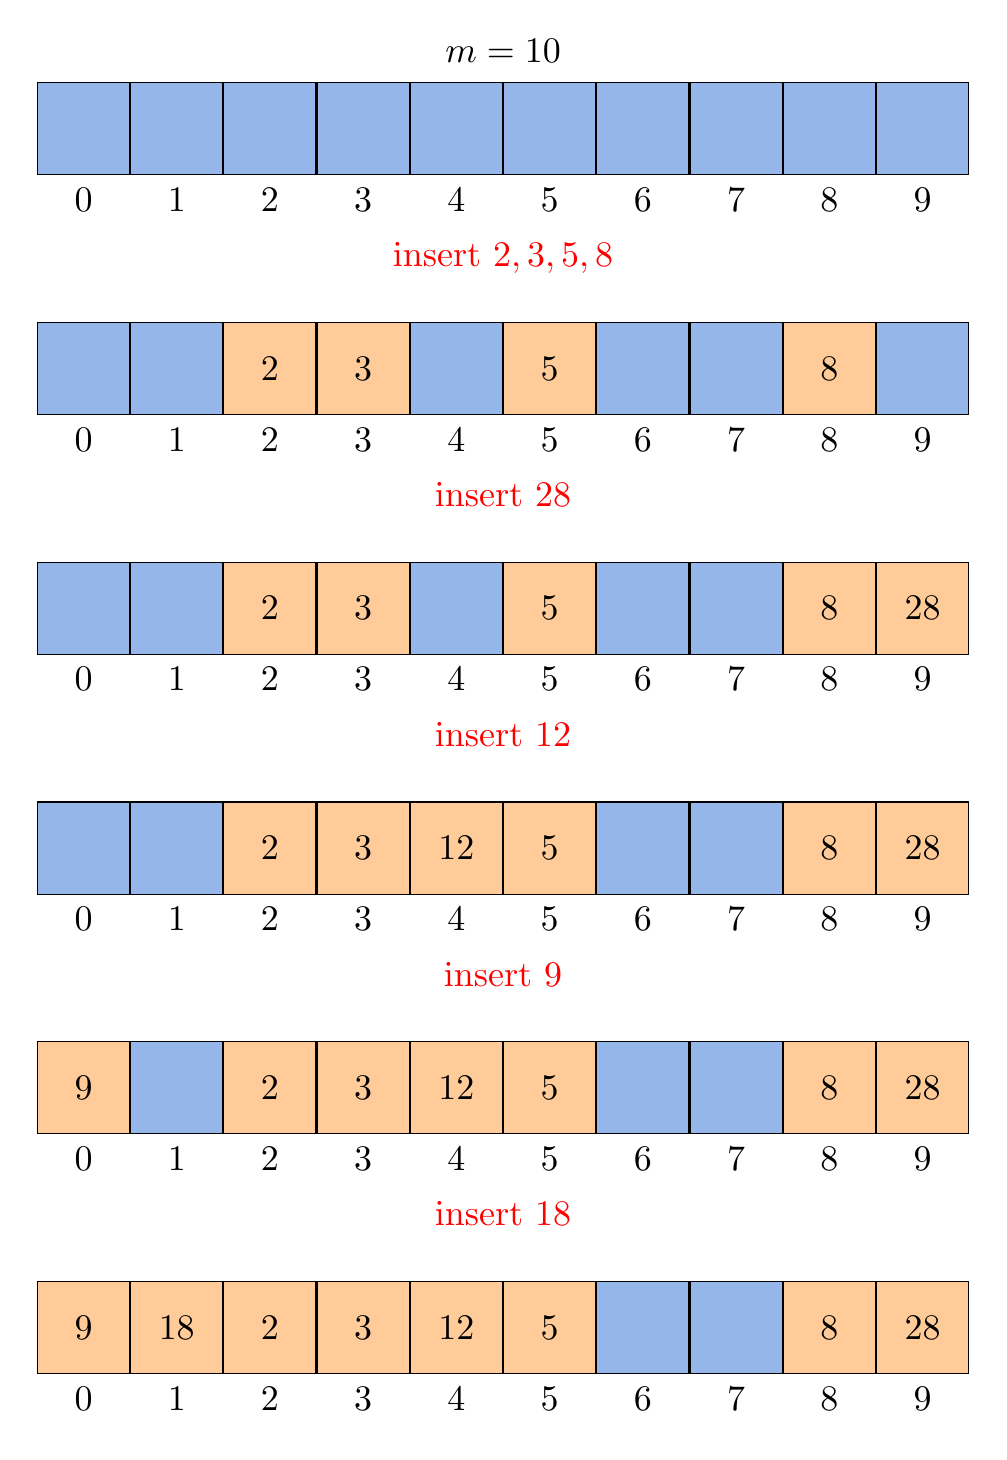
\begin{tikzpicture}[every node/.style={scale=1.3}, dot/.style={minimum size=0.1mm, circle, fill=black!90}, slot/.style={minimum size=0.9cm, rectangle}, noslot/.style={slot, fill=allcolor},
    yesslot/.style={slot, fill=orange!40}, data/.style={minimum size=0.7cm, fill=orange!40}, >=Stealth]
    \tikzstyle{textbf} = [text width=5cm,text centered]

    \matrix [row sep=1cm,nodes=draw] (table0)
    {
      \node[noslot, label=below:$0$] {}; &
      \node[noslot, label=below:$1$] {}; &
      \node[noslot, label=below:$2$] {}; &
      \node[noslot, label=below:$3$] {}; &
      \node[noslot, label=below:$4$] {}; &
      \node[noslot, label=below:$5$] {}; &
      \node[noslot, label=below:$6$] {}; &
      \node[noslot, label=below:$7$] {}; &
      \node[noslot, label=below:$8$] {}; &
      \node[noslot, label=below:$9$] {}; &
      \\
    };

    \node [above=of table0, yshift=-0.8cm]{$m = 10$};

    \node [below=of table0, red, yshift=0.8cm] {insert $2, 3, 5, 8$};

    \matrix [row sep=1cm,nodes=draw, below=of table0] (table1)
    {
      \node[noslot, label=below:$0$] {}; &
      \node[noslot, label=below:$1$] {}; &
      \node[yesslot, label=below:$2$] {2}; &
      \node[yesslot, label=below:$3$] {3}; &
      \node[noslot, label=below:$4$] {}; &
      \node[yesslot, label=below:$5$] {5}; &
      \node[noslot, label=below:$6$] {}; &
      \node[noslot, label=below:$7$] {}; &
      \node[yesslot, label=below:$8$] {8}; &
      \node[noslot, label=below:$9$] {}; &
      \\
    }; 
    \node [below=of table1, red, yshift=0.8cm] {insert $28$};

    \matrix [row sep=1cm,nodes=draw, below=of table1] (table2)
    {
      \node[noslot, label=below:$0$] {}; &
      \node[noslot, label=below:$1$] {}; &
      \node[yesslot, label=below:$2$] {2}; &
      \node[yesslot, label=below:$3$] {3}; &
      \node[noslot, label=below:$4$] {}; &
      \node[yesslot, label=below:$5$] {5}; &
      \node[noslot, label=below:$6$] {}; &
      \node[noslot, label=below:$7$] {}; &
      \node[yesslot, label=below:$8$] {8}; &
      \node[yesslot, label=below:$9$] {28}; &
      \\
    }; 

    \node [below=of table2, red, yshift=0.8cm] {insert $12$};

    \matrix [row sep=1cm,nodes=draw, below=of table2] (table3)
    {
      \node[noslot, label=below:$0$] {}; &
      \node[noslot, label=below:$1$] {}; &
      \node[yesslot, label=below:$2$] {2}; &
      \node[yesslot, label=below:$3$] {3}; &
      \node[yesslot, label=below:$4$] {12}; &
      \node[yesslot, label=below:$5$] {5}; &
      \node[noslot, label=below:$6$] {}; &
      \node[noslot, label=below:$7$] {}; &
      \node[yesslot, label=below:$8$] {8}; &
      \node[yesslot, label=below:$9$] {28}; &
      \\
    }; 

    \node [below=of table3, red, yshift=0.8cm] {insert $9$};

    \matrix [row sep=1cm,nodes=draw, below=of table3] (table4)
    {
      \node[yesslot, label=below:$0$] {9}; &
      \node[noslot, label=below:$1$] {}; &
      \node[yesslot, label=below:$2$] {2}; &
      \node[yesslot, label=below:$3$] {3}; &
      \node[yesslot, label=below:$4$] {12}; &
      \node[yesslot, label=below:$5$] {5}; &
      \node[noslot, label=below:$6$] {}; &
      \node[noslot, label=below:$7$] {}; &
      \node[yesslot, label=below:$8$] {8}; &
      \node[yesslot, label=below:$9$] {28}; &
      \\
    }; 

    \node [below=of table4, red, yshift=0.8cm] {insert $18$};

    \matrix [row sep=1cm,nodes=draw, below=of table4] (table5)
    {
      \node[yesslot, label=below:$0$] {9}; &
      \node[yesslot, label=below:$1$] {18}; &
      \node[yesslot, label=below:$2$] {2}; &
      \node[yesslot, label=below:$3$] {3}; &
      \node[yesslot, label=below:$4$] {12}; &
      \node[yesslot, label=below:$5$] {5}; &
      \node[noslot, label=below:$6$] {}; &
      \node[noslot, label=below:$7$] {}; &
      \node[yesslot, label=below:$8$] {8}; &
      \node[yesslot, label=below:$9$] {28}; &
      \\
    }; 

\end{tikzpicture}
\end{document}